 \documentclass[a4paper,12pt]{report}

%Packages Used
\usepackage{amssymb,latexsym,amsmath}     % Standard packages
\usepackage{setspace}
\usepackage{sectsty}
\usepackage{titlesec}
\usepackage{hyperref}
\usepackage{bookmark}
\usepackage{graphics,graphicx}
\usepackage{tikz}
\usepackage{mathtools}
\usepackage{graphicx}
\usepackage{esvect}

\DeclarePairedDelimiter\abs{\lvert}{\rvert}%
\DeclarePairedDelimiter\norm{\lVert}{\rVert}%

\usepackage{url,graphicx,enumitem}


%   Article style enumerate

\renewcommand{\labelenumi}{\theenumi.}

\newcommand{\R}{\mathbb{R}}
\newcommand{\Z}{\mathbb{Z}}
\newcommand{\N}{\mathbb{N}}

\newcommand{\bull}{\ensuremath{\bullet}}

\newcommand{\vc}[1]{\vec{#1}}

\newcommand{\transpose}{\mathsf{T}}

\newcommand{\lcm}{\mathrm{lcm}}
\newcommand{\ud}{\mathrm{d}}

\bookmarksetup{
  numbered,
  open
}
\renewcommand*{\thesection}{\arabic{section}}
\onehalfspacing

%Margins
\addtolength{\textwidth}{1.0in}
\addtolength{\textheight}{1.00in}
\addtolength{\evensidemargin}{-0.75in}
\addtolength{\oddsidemargin}{-0.75in}
\addtolength{\topmargin}{-.50in}

%%%%%%%%%%%%%%%%%%%%%%%%%%%%%% 
% Theorem/Proof Environments %
%%%%%%%%%%%%%%%%%%%%%%%%%%%%%%
\newtheorem{theorem}{Theorem}
\newenvironment{proof}{\noindent{\bf Proof:}}{$\hfill \Box$ \vspace{10pt}}
\sectionfont{\fontsize{12}{15}\selectfont}
\titlespacing*{\section}{0.5pt}{0.25\baselineskip}{0.25\baselineskip}


\begin{document}
\noindent
Yufei Lin

\noindent
Problem Set 7

\noindent
Nov \(14^{th}\) 2019

\begin{center}
\textbf{Problem Set 7}
\end{center}

\noindent
\textbf{Question 1}

\noindent
Suppose that $f:\R\to\R$,
$g:\R\to\R$, and $F:\R\to\R$, suppose that $f$
and $g$ are differentiable, and suppose
that
\[
f'=F
\]
and 
\[
g'=F.
\]
Then there exists a $c\in\R$ such that
\[
\forall x\in\R:\quad g(x)=f(x)+c.
\]

\noindent
\textbf{Proof: }

\noindent
Suppose $f'=F$ and $g'=F$. Thus, we have $f'-g'=(f-g)'=F-F=0$. Therefore, $f-g=c$. Then, we know $f(x)=g(x)+c$.\\

\noindent
\textbf{Question 2}

\noindent
Suppose that $f:\R\to\R$ is
differentiable, and suppose that
\[
\forall x\in\R: f'(x)=0.
\]
Then prove that there exists a $c\in\R$ such that
\[
\forall x\in\R: f(x)=c.
\]

\noindent
\textbf{Proof: }

\noindent
Suppose $f'(x)=0$. Then by mean value theorem, given $a,b \in \mathbb{R}, a<b$ such that there exists $c, f'(c)=\frac{f(b)-f(a)}{b-a}$. Therefore, if $f'(x)=0$, then $f(b)-f(a)=0$.  Thus, $f(b)=f(a)$. This means $f(x)$ is constant. $f(x)=c$. 

\pagebreak
\noindent
\textbf{Question 3}

\noindent
Suppose that $f:\R\to\R$ is
differentiable, and suppose that $a,b\in\R$, 
with $a<b$. Then there exists a $c\in\R$
such that
\[
f'(c)=\frac{f(b)-f(a)}{b-a}.
\]

\noindent
\textbf{Proof: }

\noindent
Suppose $a,b\in \mathbb{R}$, and $f(x)$ is differentiable $\forall x, x\in \mathbb{R}$. Therefore, we could have the following graph:

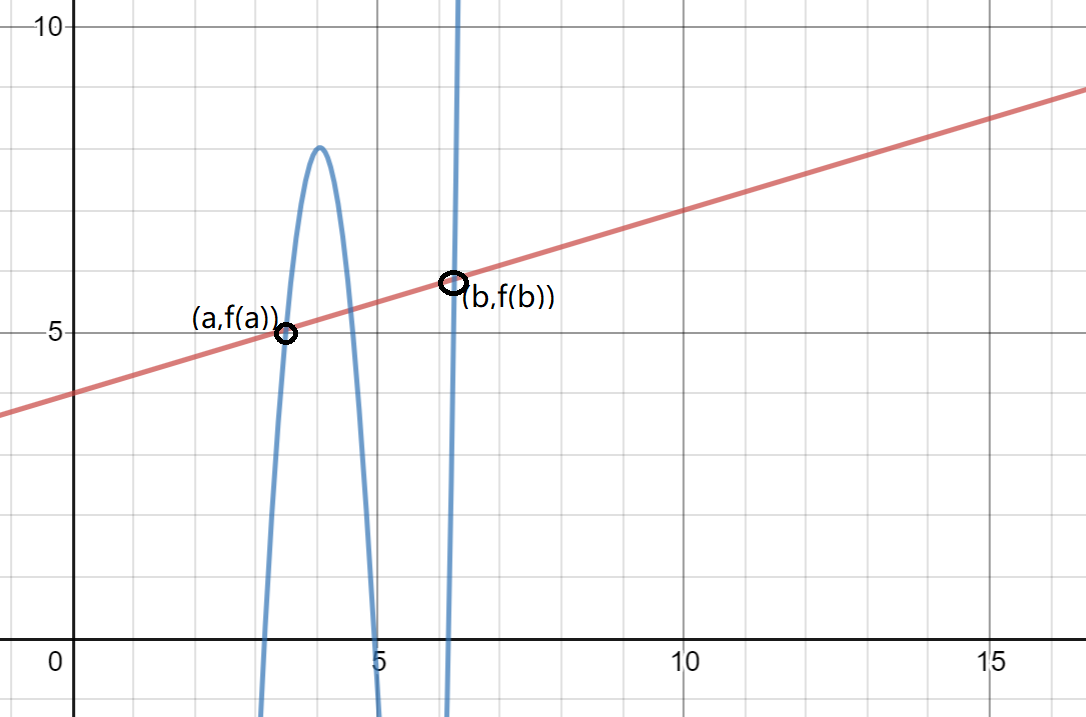
\includegraphics{Question3.png}

\noindent
Thus, we can show that if we can find a straight line function such that $(a,f(a))$ and $(b,f(b))$ is on the graph we can thus proof if the slope exist then, there must be a $f'(c)$ exist such that $f'(c)=\frac{f(b)-f(a)}{b-a}$.

\noindent
Let the straight line's function be $h(x)$, then $h(x)=\frac{f(b)-f(a)}{b-a}\cdot{x}+t, t\in \mathbb{R}$. Since $h(a)=f(a),h(b)=f(b)$ then, $h(x)=\frac{f(b)-f(a)}{b-a}\cdot{x}+\frac{b(f(a))-a(f(b))}{b-a}$. Then we have $g(x)=f(x)-h(x)$. $g(a)=g(b)=0$. Thus, by Rolle's theorem, if $g(a)=g(b)=0$ then, $\exists c,$ such that $g'(c)=0$. Then, we have $g'(c)=f'(c)-h'(c)=f'(c)-\frac{f(b)-f(a)}{b-a}=0$. Therefore,$f'(c)=\frac{f(b)-f(a)}{b-a}$. 

\pagebreak
\noindent
\textbf{Question 4}

\noindent
Suppose that $f:\R\to\R$ is
differentiable, and suppose that $a,b\in\R$, 
with $a<b$. Suppose also 
that $f(a)=f(b)$. Then there exists a $c\in\R$
such that
\[
f'(c)=0.
\]

\noindent
\textbf{Proof: }

\noindent
\textbf{(I) Maximum inside the range} 

\noindent
Suppose $a<b$, and $f:\R\to\R$ is differentiable, then there must be a $c\in [a,b]$ such that $f(c)\geq f(x),\forall x, x\in [a,b]$. Thus, we have a local maximum in range $[a,b]$. Based on Question 5, we know that if we have a local maximum at $c$, then $f'(c)=0$.

\noindent
\textbf{(II) Maximum at the end of the range}

\noindent
Suppose $a<b$, and $f:\R\to\R$ is differentiable, and we have $f(a)=f(b)$ and both of them are the maximum within the range. Since $a,b$ are the maximum point of the function in that range, then there must exist a $c$ such that $f(c)$ is the smallest within the range. Also, we know that $f$ is differentiable everywhere. Then we have $\displaystyle{\lim_{h\to 0}}\frac{f(c+h)-f(c)}{h}$ exist and $\displaystyle{\lim_{h\to 0+}}\frac{f(c+h)-f(c)}{h}=\displaystyle{\lim_{h\to 0-}}\frac{f(c+h)-f(c)}{h}$. On the left hand side of the above equality, because we know $f(c+h)>f(c)$, we have a positive numerator and a positive $h$. Then, $\displaystyle{\lim_{h\to 0+}}\frac{f(c+h)-f(c)}{h}\geq 0$. For the right hand side, we know $f(c-h)>f(c)$, then $\displaystyle{\lim_{h\to 0-}}\frac{f(c+h)-f(c)}{h}\leq 0$. Since left hand side is equal to the right hand side, we have $f'(c)=0$.\\

\noindent
\textbf{Question 5}

\noindent
Suppose that $f:\R\to\R$
has a local maximum at $c\in\R$, and suppose 
that $f$ is differentiable at $c$. Then
we have
\[
f'(c)=0.
\]

\noindent
\textbf{Proof: }

\noindent
Suppose $f$ is differentiable at $c$ and $f(c)$ is a local maximum. Then, we know $\displaystyle{\lim_{h\to 0}}\frac{f(c+h)-f(c)}{h}$ exist and $\displaystyle{\lim_{h\to 0+}}\frac{f(c+h)-f(c)}{h}=\displaystyle{\lim_{h\to 0-}}\frac{f(c+h)-f(c)}{h}$. Therefore, we should be looking at the two sides of this local maximum. Such that we will have $\displaystyle{\lim_{h\to 0+}}\frac{f(c+h)-f(c)}{h}$. The numerator is negative because $f(c)$ is local maximum, and $h$ is positive. Then, we know $\displaystyle{\lim_{h\to 0+}}\frac{f(c+h)-f(c)}{h}\leq 0$. On the other hand, $\displaystyle{\lim_{h\to 0-}}\frac{f(c+h)-f(c)}{h}$. The denominator is negative because $f(c)$ is local maximum, and $h$ is negative. Then, we have $\displaystyle{\lim_{h\to 0-}}\frac{f(c+h)-f(c)}{h}\geq 0$. Thus, $\displaystyle{\lim_{h\to 0}}\frac{f(c+h)-f(c)}{h} = 0$. \\

\noindent
\textbf{Question 6}

\noindent
Suppose that $f:\R\to\R$,
and $a\in\R$. Then the limit of $f$ at $a$ exists
and equals $L$ if, and only if, both the 
right- and left-handed limits of $f$ at $a$ 
exist and they both equal $L$.

\noindent
\textbf{Proof: }

\noindent
Suppose $\displaystyle{\lim_{x\to a}}f(x)=L$. Then, $\forall \epsilon>0, \exists \delta>0$, such that if $0<|x-a|<\delta$, then $|f(x)-L|<\epsilon$. 

\noindent
\textbf{(I)}Look at the right-handed limit first: 

\noindent
If $a<x<a+\delta$, then we have $0<|x-a|<\delta$. Therefore, $|f(x)-L|<\epsilon$.

\noindent
\textbf{(II)} Look at the left-handed limit:

\noindent
If $a>x>a-\delta$, then we have $0<|x-a|<\delta$. Therefore, $|f(x)-L|<\epsilon$.

\noindent
Therefore, if $\displaystyle{\lim_{x\to a}}f(x)=L$, then both the 
right- and left-handed limits of $f$ at $a$ 
exist and they both equal $L$.

\noindent
Conversely, suppose $\displaystyle{\lim_{x\to a+}}f(x)=\displaystyle{\lim_{x\to a-}}f(x)=L$. Then we know that $\forall \epsilon >0, \exists \delta_1>0$, such that if $a<x<a+\delta_1$, then $|f(x)-L<\epsilon|$ and $\forall \epsilon >0, \exists \delta_2>0$, such that if $a-\delta_2<x<a$, then $|f(x)-L<\epsilon|$. Let $\delta=min(\delta_1,\delta_2)$. Then we can have $\forall \epsilon$, if $a<x<a+\delta$, then $|f(x)-L<\epsilon|$ and if $a-\delta<x<a$, then $|f(x)-L<\epsilon|$. Therefore, if $0<|x-a|<\delta$, then $|f(x)-L|<\epsilon$. 

\noindent
Thus, $\displaystyle{\lim_{x\to a}}f(x)=L$ if and only if both right-handed and left-handed limit has the same value.
\end{document}